\begin{comment}
\section{Introduction}

\section{Bridge Health Monitoring}

\section{Wireless Sensor Networks and LoRa}
Wireless Sensor Networks (WSNs) are simple, low-cost networks that primarily consist of nodes and a base station \cite{WSN-WaterQual}. WSN nodes usually comprise of some sensing or measuring capability and relay this information via uplink to a base station for processing and then to a network server. Innovating many field of industry and research, these distributed networks of nodes have been valuable in many contexts. For example, the use of ZigBee communication technology for air pollution monitoring \cite{ZigBeeAirPolution} and the use of Bluetooth for communication between end-devices measuring temperature, luminance, carbon dioxide and humidity for energy-saving establishments \cite{BTenergySaving}. Although these WSNs have worked in the past, the future of this technology lies in developing systems that have high scalability and range, something that ZigBee and Bluetooth inherently lack. Cellular and satelite .... space study ... somewhere 

Long Range (LoRa) technology was introduced 

\section{The Internet of Things and LoRaWAN}
The configuration of WSNs have typically been a deployment of Wireless Personal Area Network (WPAN) or Low Power Wide Area Network (LPWAN) standards, where nodes are setup in a mesh layout using a short-range communication protocol such as ZigBee and Bluetooth \cite{WSN-WaterQual}. The main implication with these protocols is that the mesh implementation inherently bottlenecks scalability due to exponentially increasing network requirements and power consumption \cite{IOTandLORAWAN-SmartFarm}. Long Range Wide Area Network (LoRaWAN) is a solution to implementing an LPWAN system with minimal complexity and scalability whilst also being low power. LoRa by definition is a chirp spread spectrum (CSS) modulation technique developed by Cycleo offering a Medium Access Control (MAC) layer protocol and operates on the `licence-free region-dependent industrial, scientific, and medical (ISM) frequncy bands' \cite{IOTandLORAWAN-SmartFarm}. In Australia the operational ISM band for LoRa is between 915 and 928 MHz. LoRaWAN is the ideal technology for agritulcutral and regional purposes due to its long range, low power and long lifetime. 
\end{comment}

\section{Review of the Published Literature}
This literature review analyses the works already conducted in the field of WSNs and LoRaWAN communication protocol in terms of signal strength, IoT architecture and security. The relation of this report in regards to the existing literature will be discussed. 

Gehani et al. in 2021 \cite{LoRa-Agro-Informatics} implements a LoRaWAN IoT architecture for measuring Agro-Informatics regarding the detection and classification of pathogens affecting the roots of plants. The signal strength of the LoRa packet was measured in terms of received signal strength indication (RSSI) and signal-to-noise ratio (SNR) in various depths between 0 cm to 60 cm. The experimental setup consisted of a simple transmission and receiving Adafruit Feather M0 microcontrollers using an RFM95W based LoRa radio transceiver operating on the US915 MHz frequency. A rechargeable 3.7 lithium polymer 500 mAh battery was used for the power supply and a ceramic antenna was used for the buried microcontroller. The transmitting node was initially placed inside a bucket containing dry soil, and the receiving node placed 3 m away logged the RSSI and SNR for ten LoRa packets. A diagram of the experimental setup is shown in figure \ref{lora-bucket}. 

\begin{figure}[h]
	\centering
	\caption{Experimental Setup for LoRa Node in Soil \cite{LoRa-Agro-Informatics}}
	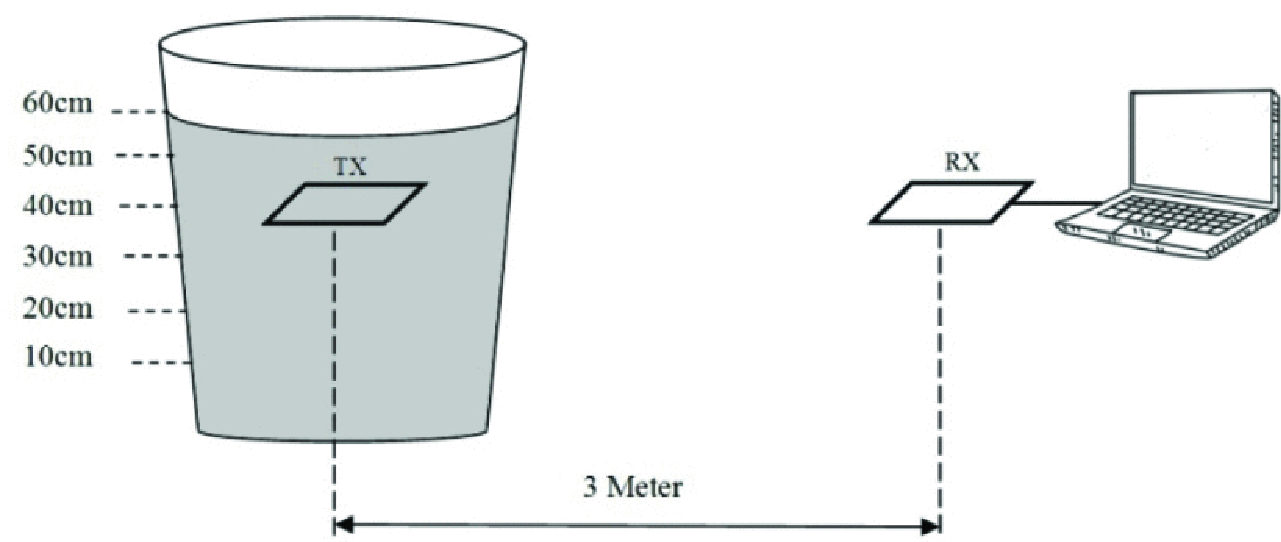
\includegraphics[scale=0.5]{Sections/Literature-Review/Lora-bucket.pdf}
	\label{lora-bucket}
\end{figure}

The results conclude that the LoRa transmitter was capable of transmitting packets when buried within 60 cm with the recommendation that depth does not exceed 50 cm. The depth of the transmitter node proved to be inversely proportional to the RSSI value which did not drop below the minimum signal power required for demodulation. The results of the depth transmission in this study are helpful in deducing appropriate enclosure thickness for the purposes of this report.

\begin{comment}
Wixted et al. in 2016 \cite{LoRa-WSN} evaluates the indoor and outdoor performance of the LoRaWAN physical layer and network layer across the central business district (CBD) of Glasgow city, Scotland. The LoRaWAN testing involved the implementation of Multitech mDot devices which comprised of a LoRa wireless chip and ARM processor. These nodes interfaced with a Raspberry Pi via USB which was used to record the current location. A cabled gateway and two gateways using mobile connections were placed at the top of three buildings. The LoRa nodes were configured via the Stream Technologies IoT platform, acting as the application layer, and the nodes transmitted packets in which successful or failed acknowledgements (ACK)s were logged. Data was collected by walking through the city streets and the data from the network server was logged in a database. 
The reliability experimental setup involved nodes repeatedly sending messages over a long period of time and iterating over multiple spreading factor (SF)s. In this scenario the node was placed 1.9 km from one gateway an 2.1 km from a second gateway. 

The results of the LoRaWAN performance indicate that in several trouble spots, such as a 100 m pedestrian underpass, the GPS failed to operate but LoRaWAN was able to continue communication. Additionally, the multi-gateway setup meant that many locations were detected by more than just one gateway.

Figure \ref{LoRaWAN-performance-testing} displays the experimental results with markers indicating ---


The results of the reliability testing indicate that the 
\end{comment}

Fox et al. in 2019 \cite{IoT-Regional-Service} presents the design architecture for a LoRaWAN based IoT system for services a local region in Ireland. The IoT architecture in this study consisted of an Arduino Pro Mini as an end-device powered by two double A batteries. A Multiconnect Conduit IP67 was chosen as the gateway, using a 3dBi dipole antenna. The IBM cloud platform was deployed using an MQTT broker as the backend. 
